\chapter{Knowledge Base Population}
\label{chap:kbp}

Since my methods can only be evaluated through well defined tasks, I chose multiple challenges where measuring the accuracy of my models can be verified. This chapter includes the task of Knowledge base population which goal is to discover facts about entities and augment a knowledge base with these facts. In this challenge we achieved a high accuracy of generating millions of new facts only using simple inference rules. After that, in the next Chapter, I will discuss my experiments with Natural language inference, where I will introduce my method of measuring support score of the concept graphs, and defining new inference rules to enhance the expansion method, generating a more abstract version. Next my baseline to the NLI task is discussed, followed by the review of my problems with the \textit{MultiNLI} dataset \footnote{\url{https://www.nyu.edu/projects/bowman/multinli/}}. Finally I explain the machine comprehension challenge, and I will introduce my baseline method for solving it, using my micro-service for automatically building concept graphs. After that I will present how we made it possible to integrate it to an already working system that uses deep learning algorithms.

%----------------------------------------------------------------------------
\section{Introduction} 
The first task I chose to evaluate my models on was the Knowledge base population challenge. Here I present a set of pilot experiments for augmenting a generic, open-domain 
knowledge base using a graph-based lexical ontology of English and simple
inference rules. The WikiData knowledge-base contains facts encoded as relation
triplets, such as author(George Orwell, 1984), based on which naive
speakers can easily establish additional facts such as that George Orwell is a
person and 1984 is some written work, most likely a book. To automate this type
of inference we need models of lexical semantics that are more explicit than
the distributional models commonly used in computational semantics. For this I used my REST-API built on the \textbf{4lang} formalism to automatically build concept graphs. The representation of "author" will likely contain edges
corresponding to facts such as \texttt{IS\_A(author, person)} and
\texttt{write(author, book)}.
I define simple templates that use these representations for inference over
WiktData facts. My method yields millions of new facts with high
accuracy (over 90\% according to manual evaluation)

\section{Background}
\texttt{WikiData}\footnote{\url{https://www.wikidata.org/}}
is a public domain knowledge base containing
attribute-value type information about more than 30 million entities.
For each entity, WikiData contains pairs of \textit{properties}
(attribute) and \textit{values}, which may contain pointers to other
entities. In case of the entity \texttt{1984}, the value of the property
\texttt{author} is \texttt{George\_Orwell}. An alternative
representation of the dataset is in the form of relational triplets,
this would represent the above fact as a single binary relation
\texttt{author(George\_Orwell, 1984)}. I use This latter representation
when processing WikiData and use the \textbf{4lang} service to process this set of
definition graphs when performing inference over WikiData triplets. These triplets can be generated from the \textit{json} format of the dataset, which is online accessible. The first step I had to take was to preprocess the raw dataset to obtain the triplets format. For this I used python language as well.

\section{Method}
Two simple patterns were implemented for performing inference using
\texttt{WikiData}
triplets and \texttt{4lang} definitions. Given the triplet
\texttt{author(George\_Orwell, 1984)} and the definition graph
of \texttt{author} in Figure~\ref{fig:author}, it should be doable to
infer all edges in the graph in Figure~\ref{fig:orwell_inf}. This
requires an implementation of two patterns. Given a triplet $R(X, Y)$, I
first found nodes in the \texttt{4lang} definition of $R$ that are connected
to $R$ by an outgoing 0-edge (e.g. \texttt{author} $\xrightarrow0$
\texttt{write}) and assumed that each of these 0-relations holds for $X$.
The second inference I would like to make is \texttt{1984}~$\xrightarrow0$~book
based on the \texttt{4lang} edge \texttt{write} $\xrightarrow2$ book. To this end
I implemented the rule that if for any relation $R$ and concepts $B$ and $C$
I found $R \xrightarrow0 B \xrightarrow2 C$, then for each triplet $R(X, Y)$ I
added the edge $Y \xrightarrow0 C$. 

An issue I encountered early concerns words with multiple outgoing
0-edges in their definition graph. Often, this is the result of a
dictionary definition that lists several categories that the concept may
belong to, e.g. the definition of \texttt{employer} is \textit{a person,
	company, or organization that employs people}. In case of a triplet such
as \texttt{employer(CIA, Mike\_Pompeo)}, the incorrect inference
\texttt{CIA} $\xrightarrow0$ \texttt{person} would be made. Special treatment for such
constructions by \textbf{4lang} and/or my system might handle these cases and
make the inference that the CIA is either a person, a company, or an
organization, but for the purpose of the present experiment I decided
to discard all \texttt{WikiData} relations whose \texttt{4lang}
definition contains more than one outgoing 0-edge.

Other issues are caused by meaningless or erroneous 0-connections in 4lang graphs
that are ultimately limitations of the method used by the \texttt{dict\_to\_4lang}
system to build these graphs from natural language definitions. The process involves parsing
the definitions with a state-of-the-art dependency parser and mapping grammatical
relations between pairs of words to configurations of \texttt{4lang} edges.
In case of a definition such as \textbf{flag:}
\textit{piece of cloth with a coloured pattern or picture on it that represents
	a country}, the definition graph will contain the edge
\texttt{flag} $\xrightarrow0$ \texttt{piece}. This information
is obviously not informative (to say the least), we consider it an error
when evaluating my system.
To make a correct inference about flags similar to those in our previous example,
a system would need to learn something along the lines of
``\textit{piece of X} $\xrightarrow0$ \texttt{X}'', which is beyond the scope of
the current thesis. 
A final common source of false facts concerns words that are used in WikiData
in a very different sense than the one defined by the Longman dictionary, the source
of \texttt{4lang} definitions. One example is the outdated definition of
\texttt{developer}: \textit{a person or company that makes money by buying land
	and then building houses, factories etc on it}, which causes our method to erroneously
infer that developers are companies.

\begin{figure}
	\centering
	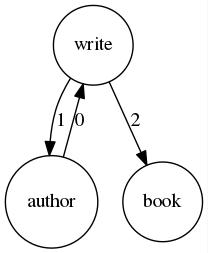
\includegraphics[scale=0.5]{figures/author.jpg}
	\caption{4lang definition of \texttt{author}.}
	\label{fig:author}
\end{figure}

\begin{figure}
	\centering
	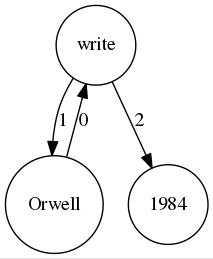
\includegraphics[scale=0.5]{figures/orwell_inf.jpg}
	\caption{4lang graph produced from WikiData triplet
		\texttt{author(George\_Orwell, 1984)}.}
	\label{fig:orwell_inf}
\end{figure}

\subsection{Evaluation}

In the WikiData dataset first I counted the triplets. I found 86.3 million triplets using 893 unique predicates.
I started our experiment by preprocessing WikiData to discard fragmentary data
(triplets with empty positions) and multi-word predicates that do not lend themselves
to the simple methods described in the previous section. This was made by python code, and is available on github \footnote{\url{https://github.com/adaamko/4lang}}.
After these steps the dataset consisted of 195 predicates and 19.6 million triplets,
out of which the first inference pattern was applicable to 108 predicates
(covering 9.2 million triplets), the second to 27 predicates (covering 1.4 million triplets).
After an initial examination of the output I decided to discard further subsets
of predicates: I applied our patterns to predicated whose definition graphs had exactly one outgoing
0- or 2-edge and no incoming edges. This step resulted in a considerable increase in
overall accuracy. After these steps I proceeded to apply our two patterns: the first one was
now applicable to 84 predicates (8.2 million triplets), the second to 25 predicates (0.8 million triplets).
This relatively small number of unique predicates allowed to inspect all of them manually and estimate the quality of all newly
extracted facts: if we find that for some predicate, e.g. \texttt{father}, I
have made inferences based on the template ``$X \xrightarrow0$ \texttt{father}
implies $X \xrightarrow0$ \texttt{male}'', it assumes that each fact inferred
using this template is correct, while for erroneous templates I assume that
each extracted fact is false. Figures are shown in Table~\ref{table:results}.
Note that our evaluation
was strict in the sense that we judged incorrect all non-informative edges, e.g.
$X~\xrightarrow0$~\texttt{something}.

\begin{table}
	\centering
	\begin{tabular}{lrrr}
		& 1-pattern & 2-pattern & total\\
		predicates  & 84 & 25 & 109 \\
		correct     & 55 & 17 & 72 \\
		new facts   & 8.2 million & 0.83 million & 9 million \\
		correct     & 7.6 million & 0.74 million & 8.3 million \\ 
		accuracy    & 0.92 & 0.89 & 0.92
	\end{tabular}
	\caption{Evaluation results}
	\label{table:results}
\end{table}

This pilot system presented here used simple pattern-based
methods for combining facts from a knowledge base with linguistic knowledge
represented in a lexical ontology. We believe
the significance of this experiment lies not in its yield of millions of high-quality
facts with which a knowledge base might be extended, but in its demonstration
that inference based on linguistic knowledge is a powerful
method for enriching any natural language data. In the next chapter I will discuss the NLI challenge, and my methods of measuring similarity between concept graphs.